


% ----------------------------------------------------------------------------
% Syntax-Abkürzungen für logische und mengentheoretische Operatoren
% ----------------------------------------------------------------------------
% Dieser Abschnitt definiert Kurzformen (Abkürzungen) für häufig verwendete logische
% und mengentheoretische Operatoren, die in diesem Dokumentin Form von Commands 
% verwendet werden. Diese Kurzformen sind entworfen, um die Lesbarkeit des Codes zu 
% verbessern und eine effiziente Bearbeitung zu ermöglichen.
%
% ----------------------------------------------------------------------------
\usepackage{tikz}

    \newcommand{\rA}{\hyperref[rule:A]{\ensuremath{A}}}
    % Regeln zum Umgang mit dem ∧-Symbol
    \newcommand{\rAI}[1]{\hyperref[rule:AI]{\ensuremath{\land}I(#1)}}
    \newcommand{\rAEa}[1]{\hyperref[rule:AE1]{\ensuremath{\land}E1(#1)}}
    \newcommand{\rAEb}[1]{\hyperref[rule:AE2]{\ensuremath{\land}E2(#1)}}
    \newcommand{\rAEn}[1]{\hyperref[rule:AEn]{\ensuremath{\land}E(#1)}}	
	
    % Regeln zum Umgang mit dem ∨-Symbol
    \newcommand{\rOIa}[1]{\hyperref[rule:OI1]{\ensuremath{\lor}I1(#1)}}
    \newcommand{\rOIb}[1]{\hyperref[rule:OI2]{\ensuremath{\lor}I2(#1)}}
    \newcommand{\rOE}[1]{\hyperref[rule:OE]{\ensuremath{\lor}E(#1)}}	
    \newcommand{\rOEn}[1]{\hyperref[rule:OEn]{\ensuremath{\lor}E(#1)}}	
	
    % Regeln zum Umgang mit dem →-Symbol
    \newcommand{\rRI}[1]{\hyperref[rule:RI]{\ensuremath{\rightarrow}I(#1)}}	
    \newcommand{\rRE}[1]{\hyperref[rule:RE]{\ensuremath{\rightarrow}E(#1)}}	
	
    % Regeln zu Umgang mit dem ↔.Symbol
    \newcommand{\rLRI}[1]{\hyperref[rule:LRI]{\ensuremath{\leftrightarrow}I(#1)}}	
    \newcommand{\rLREa}[1]{\hyperref[rule:LRE1]
    {\ensuremath{\leftrightarrow}E1(#1)}}	
    \newcommand{\rLREb}[1]{\hyperref[rule:LRE2]{\ensuremath{\leftrightarrow}E2(#1)}}

    \newcommand{\rLRS}[1]{\hyperref[rule:LRSubst]{\ensuremath{\leftrightarrow}S(#1)}}

	
    % Regeln zum Umgang mit dem ∀-Symbol
    \newcommand{\rUI}[1]{\hyperref[rule:UI]{\ensuremath{\forall}I(#1)}}		
    \newcommand{\rUE}[1]{\hyperref[rule:UE]{\ensuremath{\forall}E(#1)}}	
	
	
    % Regeln zum Umgang mit dem ∃-Symbol	
    \newcommand{\rEI}[1]{\hyperref[rule:EI]{\ensuremath{\exists}I(#1)}}				
    \newcommand{\rEE}[1]{\hyperref[rule:EE]{\ensuremath{\exists}E(#1)}}	
	
    % Regeln zum Umgang mit dem ∃!-Symbol
    \newcommand{\UEI}[1]{\hyperref[rule:UEI]{\ensuremath{\exists!}I(#1)}}			
    \newcommand{\UEE}[1]{\hyperref[rule:UEE]{\ensuremath{\exists!}E(#1)}}	

    % Regeln zum Umgang mit dem =-Symbol
    \newcommand{\rII}{\hyperref[rule:II]{\ensuremath{=}I}}
    \newcommand{\rIE}[1]{\hyperref[rule:IE]{\ensuremath{=}E(#1)}}	

    % Regeln zum Umgang mit dem =-Symbol dreier Gleichheiten
    \newcommand{\rIIb}[1]{\hyperref[rule:rIIb]{\ensuremath{=}I(#1)}}
    \newcommand{\rIEb}[1]{\hyperref[rule:rIEb]{\ensuremath{=}E(#1)}}	
	
    \newcommand{\rNeq}{\hyperref[rule:Neq]{\ensuremath{\neq}}}	
	
    % Regeln zum Umgang mit dem ¬-Symbol als auch dem ⊥-Symbol	
    \newcommand{\rBI}[1]{\hyperref[rule:BI]{\ensuremath{\bot}I(#1)}}
    \newcommand{\rCI}[1]{\hyperref[rule:CI]{\ensuremath{\neg}I(#1)}}
    \newcommand{\rCE}[1]{\hyperref[rule:CE]{\ensuremath{\neg}E(#1)}}
    \newcommand{\rDN}[1]{\hyperref[rule:DN]{\ensuremath{}DN(#1)}}


    % Regel zur Kettennotation
    \newcommand{\rChain}[1]{\hyperref[rule:Chain]{\ensuremath{\mathsf{Tr.}}(#1)}}

    %Xor
    \newcommand*\lxor{\mathbin{\veebar}}
    
    \newcommand{\eqvdash}{\dashv\vdash}

    % Powerset
    \newcommand{\powerset}{\mathcal{P}}

    %Induktionsprinzip
    \newcommand{\rInduktion}[1]{\hyperref[rule:Induktion]{\ensuremath{\mathrm{Induktion}}(#1)}}

    %Identitätsoperator
    \newcommand{\Id}{\mathrm{id}}


    % Symbol injektiven Abbildung
    \newcommand{\inj}{\rightarrowtail}
    % Symbol surjektiven Abbildung
    \newcommand{\sur}{\twoheadrightarrow}
    % Symbol bijektiver Abbildung
    \newcommand{\bij}{\xrightarrow{\sim}}


    % eigenes Relationssymbol: Punkt mit mehreren Pfeilen nach rechts
    \newcommand{\multirel}{%
      \mathrel{%
        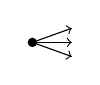
\begin{tikzpicture}[baseline=-0.6ex]
          % Punkt
          \fill (0,0) circle (0.06);
    
          % Pfeile nach rechts (Sonnenstrahlen)
          \draw[->] (0,0) -- (0.5,0);        % gerade nach rechts
          \draw[->] (0,0) -- (0.5,0.18);     % schräg nach oben rechts
          \draw[->] (0,0) -- (0.5,-0.18);    % schräg nach unten rechts
        \end{tikzpicture}%
      }%
    }



    


